
\title{Definisi GIS (GEOGRAPHICS INFORMATION SYSTEM)}
\author{Kelompok 1}
% kelompok1
% ariana setiawan (1154042)
% idang mawardi (1154084)
% arya niken manalu (1154080)
% M. Arya Sikumbang (1154075)
% r rifa fauzi komara (1154089)
% Andi Tenri Wali (1154013)

\section{Definisi GIS}
Geographical information system (GIS) adalah sebuah komputer yang berbasis sistem
informasi digunakan untuk memberikan informasi bentuk digital dan analisa terhadap 
permukaan geografi bumi.

\subsection{Pemahaman pada Geographics Information System GIS}
Dimana GIS merupakan pemahaman dari, sebagai berikut:
\begin{enumerate}
\item Geography

Dimana GIS dibangun berdasarkan pada istilah‘geografi’ atau ‘spasial’.
Object mengacu pada spesifikasi lokasi dalam suatu tempat/ruang. Objek dapat berupa fisik,
budaya ataupun ekonomi alamiah. Penampakan yang seperti ini ditampilkan pada suatu peta yang 
digunakan untuk memberikan gambaran yang lebih representatif dari spasial dari suatu objek.
sesuai dengan kenyataannya yang di bumi. Dimana simbol, warna dan gaya garis digunakan sebagai
perwakilan dari setiap spasial yang berbeda pada peta dua dimensi.
Pada gambar \ref{dataspasial} dijelaskan bahwa data spasial berikut berupa 
titik, garis, poligon (2-D) dan permukaan (3-D).

\begin{figure}[ht]
	\centerline{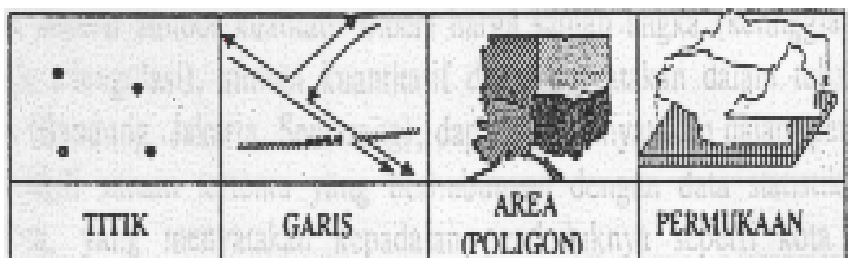
\includegraphics[width=1\textwidth]{figures/dataspasial.JPEG}}
	\caption{data spasial berikut berupa titik, garis, poligon (2-D), permukaan (3-D).}
	\label{dataspasial}
	\end{figure}

Dan arti dari gambar diatas adalah :
Format Titik 						
- Memiliki koordinat tunggal 		
- Tanpa memiliki panjang 			
- Tanpa memiliki luasan

Format Garis
- memiliki koordinat titik awal dan akhir		
- memiliki panjang tanpa luasan

Format Poligon 					
- memiliki koordinat titik awal dan akhir
-memiliki panjang dan luasan 		

Format Permukaan
- memiliki area koordinat vertikal
- memiliki area dengan ketinggian

\item Information
Informasi berasal dari kata pengolahan sejumlah data. Di dalam GIS informasi mempunyai
volume terbesar. Dan setiap object geografi memiliki setting datanya tersendiri karena 
tidak sepenuhnya data yang ada dapat terwakili didalam peta. Maka, semua data harus
diasosiasikan pada objek spasial yang mampu membuat peta menjadi intelligent.

\item System
Pengertian dari suatu sistem merupakan kumpulan elemen-elemen yang saling berintegrasi 
dan berinterdependensi dalam sebuah lingkungan yang dinamis untuk mencapai tujuan tertentu.
\end{enumerate}

\subsection{Definisi GIS (Geography Information and System)}
Dan defenisi dari GIS dapat selalu berubah karena GIS adalah bidang kajian ilmu 
dan teknologi yang masih baru. Beberapa defenisi dari Geographical Information System yaitu:
\begin{enumerate}
\item Definisi GIS menurut(Rhind, 1988):
yaitu : GIS is a computer system for collecting, checking, integrating and analyzing
information related to the surface of the earth.

\item Definisi GIS menurut(Marble \& Peuquet, 1983) and (Parker,
1988; Ozemoy et al., 1981; Burrough, 1986):
yaitu : GIS deals with space-time data and often but not necessarily, employs computer
hardware and software.

\item Difinisi GIS menurut (Purwadhi, 1994):
- SIG adalah suatu sistem yang mampu mengorganisir perangkat keras (hardware),
perangkat lunak (software), dan data, serta dapat mendaya dan digunakan sistem
penyimpanan, pengolahan, maupun analisis data yang dilakukan secara simultan, sehingga dapat
diperoleh seluruh informasi yang berkaitan secara langsung dengan aspek keruangan.
- SIG adalah manajemen data spasial dan data non-spasial yang berbasis komputer
dengan menggunakan tiga karakteristik dasar, yaitu: 
(i) memiliki fenomena yang aktual (variabel data non-lokasi) dan berhubungan 
dengan topik permasalahan di lokasi bersangkutan; 
(ii) merupakan suatu kejadian di suatu lokasi tertentu; 
(iii) memiliki dimensi waktu. Alasan GIS dibutuhkan adalah karena untuk data spasial 
penanganannya sangat sulit karena peta dan data statistik cepat mengalami kadaluarsa 
sehingga tidak ada pelayanan penyediaan data dan informasi yang diberikan menjadi tidak akurat.
\end{enumerate} 

Berikut merupakan keistimewaan analisa dengan Geographical Information System (GIS) yaitu:
\begin{enumerate}
\item Analisa Proximity
Analisa Proximity adalah geografi yang berbasis pada jarak antar layer.
Didalam analisis proximity GIS menggunakan proses yang disebut dengan buffering
yaitu membangun lapisan pendukung sekitar layer dalam jarak tertentu agar dapat menentukan
dekatnya hugungan antara sifat bagian yang ada.
\item Analisa Overlay
Analisa Overlay adalah proses integrasi data dari lapisan-lapisan layer yang berbeda (overlay).
Yang secara analisa membutuhkan lebih dari satu layer yang akan ditumpang susun secara
fisik agar dapat dianalisa secara visual.
\end{enumerate}

Maka artikel :
	Dalam sebuah artikel dari husein yang menyebutkan bahwa  GIS merupakan pemahaman dari
	Geography, Information dan System \cite{husein2006konsep}.

\section{Geographic Information System (GIS): Introduction to the computer perspective}
Sistem Informasi Geografi (GIS) diartikan sebagai sistem untuk menyimpan, memeriksa, 
mengintegrasi, memanipulasi, menganalisis dan memaparkan data yang berkaitan dengan semua 
ruang yang berhubungan dengan keadaan bumi.
Maka artikel :
	Dalam sebuah artikel dari prahasta yang menyebutkan bahwa  GIS merupakan menyimpan, memeriksa, mengintegrasi, memanipulasi, menganalisis dan memaparkan data yang berkaitan dengan semua ruang yang berhubungan dengan keadaan bumi., Information dan System \cite{prahasta2009sistem}.

\subsection{Pengenalan GIS atau Geography Information System}
1. GIS atau dikenal dengan Sistem Informasi Geografi ditunjukan sebagai sistem yang mampu menyimpan, memeriksa, mengintegrasikan, memanipulasi, menganalisis dan memaparkan data-data yang terkait dengan spasial yang merunjuk terhadap bagian bumi. (Jabatan Alam Sekitar, 1987).

2. GIS merupakan satu set lat untuk mengumpulkan, menyimpan, mendapatkan, mengubah dan memaparkan data ruang dari keadaan  bumi yang sebenarnya untuk keperluan tertentu (Burrough, 1986).

3. GIS adalah setiap set manual atau prosedur komputer yang digunakan untuk menyimpan dan memanipulasi data geografis yang tersedia (Arronoff, 1989).

4. GIS merangkum keadaan bumi dengan peranti atau perangkat tertentu yang digunakan untuk peta input atau peta produk, bersama-sama dengan dengan sistem komunikasi yang diperlukan untuk dijadikan sebagai penghubung berbagai unsur. (Star \& Ester, 1990).

5. GIS adalah suatu sistem untuk membantu dalam membangunkan model tertentu yang mustahil untuk dijadikan sintesi data yang banyak. (Martin, 1996).

\subsection{Komponen GIS atau Geography Information System}
Komponen GIS sendiri dibagikan menjadi 3 komponen, yaitu :
Sistem Komputer (perkakas dan sistem operasi), Software GIS
(ArcGIS), database GIS, methode GIS (Prosedur analisis), People (Orang-orang yang menggunakan GIS/User).
Pada gambar \ref{komponenGIS} dijelaskan bahwa kompnen GIS sebagai berikut.
\begin{figure}[ht]
	\centerline{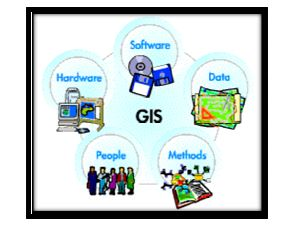
\includegraphics[width=1\textwidth]{figures/komponenGIS.JPG}}
	\caption{komponen GIS.}
	\label{komponenGIS}
	\end{figure}

\subsubsection{Komponen GIS atau Geography Information System}
sesuai dengan gambar diatas komponen GIS dibagi menjadi 3 bagian, yaitu :
1. Sistem Komputer (perkakas dan sistem operasi), merupakan hardware dari sebuah sistem GIS. Perkakas terdiri dari monitor, unit sistem atau CPU, keyboard dan mouse (Heywood et al., 2002). Teknologi komputer harus memiliki kemampuan kuasa
yang tinggi untuk menjalankan perisian GIS.

2. Software GIS , merupakan ArcGIS untuk tujuan perancangan, pengurusan ataupun pemodelan pada kebutuhan tertentu.

3. Database GIS , merupakan tempat yang melibatkan data GIS baik data spatial dan pengurusan datanya. memori untuk menyimpan jumlah data yang besar dan mempunyai kualitas yang baik dengan resolusi tinggi pada skrin grafik warna (untuk membantu dalam menentukan maklumat yang dihasilkan atau diberikan melalui penggunaan warna yang berbeda).

4. Methode GIS , merupakan prosedur dari analisis sistem GIS. yang melibatkan proses input, proses menyimpan, proses mengurus, proses menukar, proses menganalisis, dan proses output yang hanya melibatkan perisian GIS untuk mengatur sistem dan data-data tersebut (Heywood et al., 2002 )

5. People , merupakan orang-orang yang menggunakan sistem GIS. atau orang yang mengendaliakn proses input-output sistem GIS. 

\subsection{Kaedah GIS atau Geography Information System}
Berdasarkan pemahaman diatas, kaedah GIS juga merupakan salah satu komponen penting untuk mengatur sistem GIS sesuai dengan penjelasan sebelumnya. Kaedah-kaedah ini terdiri dari input
data spatial, pengurusan data atribut, paparan data, penerokaan data, analisis dan pemodelan data GIS;
yang dijelaskan oleh gambar sebagai berikut:
Pada gambar \ref{kaedahGIS} dijelaskan bahwa kaedah GIS sebagai berikut.
\begin{figure}[ht]
	\centerline{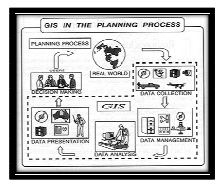
\includegraphics[width=1\textwidth]{figures/kaedahGIS.JPG}}
	\caption{kaedah GIS.}
	\label{kaedahGIS}
	\end{figure}

\subsubsection{Kaedah GIS atau Geography Information System}
1. Input data spatial
Merupakan langkah awal agar terciptanya data baru, dengan cara menginputkan data dan sistem GIS akan menyuntingnya dalam bentuk transformasi geometri yang nantinya akan menghasilkannya kedalam bentuk hard copy. (Chang, 2008) 
(Heywood et al., 2002).

2. Pengurusan data artibut
Merupakan langkah selanjutnya agar sumber peta dapat dipindahkan kepada peta digital yang dapat dibaca oleh GIS.
(Chang, 2008) (Worboy \& Duckham, 2003) (Heywood et al., 2002)

3. Pengumpulan data
Merupakan aktivitas untuk proses melakukan eksplorasi lebih jauh dalam meneliti ciri kesamaa dalam suatu graf peta yang berbeda. (Worboy \& Duckham, 2003).

4. Analisis data
Merupakan cara untuk memaparkan dan memanipulasi data yang didapat. Dengan menggunakan 2 jenis format, yaitu :
- data vektor : melibatkan beberapa kaedah seperti penimbalan / buffering, penindihan/overlay, pengukuran jarak, statik ruang, dan manipulasi peta.
- data raster : menaganalisis pengumpulan data tempatan, kaedah kejiranan, kaedah berzon, dan kaedah operasi global.
(Chang, 2008) (Worboy \& Duckham, 2003) (Heywood et al., 2002)

5. Paparan data dan output data
Dasarnya disediakan untuk tujuan pemaparan hasil dari analisis data yang fungsinya ditujukan untuk pengguna.

6. Aplikasi GIS
Digunakan untuk keperluan tertentu dan bersifat umum bagi masyarakat tergantung keperluan penggunanya. 
(Heywood et al., 2002).

Pada gambar \ref{aplikasiGIS} dijelaskan bahwa aplikasi GIS sesuai keperluan penggunan sebagai berikut.
\begin{figure}[ht]
	\centerline{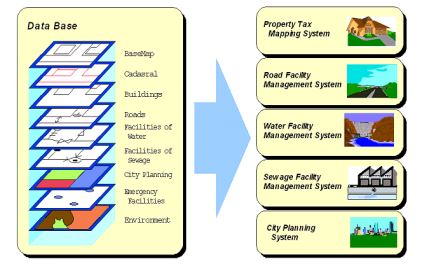
\includegraphics[width=1\textwidth]{figures/aplikasiGIS.JPG}}
	\caption{aplikasi GIS.}
	\label{aplikasiGIS}
	\end{figure}
Maka artikel :
	Dalam sebuah artikel dari hua yang menyebutkan bahwa  GIS memiliki kaedah dan komponen, Information dan System \cite{hua2017sistem}.

\subsection{Kesimpulan GIS atau Geography Information System}
Kesimpulannya, GIS merupakan alat yang penting dalam perspektif komputer pada masa kini dikarenakan GIS
mempunyai kemampuan aplikasi dalam berbagai bidang, misalnya dalam proses perancangan bandar dan kartografi,
penilaian kesan alam sekitar dan pengurusan sumber asli. GIS juga memainkan peranan dalam perspektif perniagaan,
dimana alat ini sangat bermanfaat dalam pengiklanan dan pemasaran, jualan, dan logistik 
mampu digunakan untuk mencari dan meningkatkan perniagaan seperti tapak perniagaan yang strategik. Sebagai umum, pengguna GIS dapat dilibatkan dengan agensi-agensi penguatkuasaan undang-undang, strategi
perancangan, perhutanan, industri, pemberdayaan alam, perencanaan kota, profesional
telekomunikasi, kesehatan, pengangkutan, geografi, dan pembangunan pemasaran. 
Penjelasan ini menyediakan platform untuk memahami lebih lanjut tentang komponen, kaedah, dan aplikasi GIS, 
untuk mempelajari tentang alat GIS.
\subsection{Saran GIS atau Geography Information System}
GIS dapat diaplikasikan di dalam kehidupan sehari-hari untuk memenuhi kebutuhan dan dapat membantu kebutuhan setiap masyarakat menjadi lebih baik dan lebih bermanfaat. Karena dengan memanfaatkan kemajuan teknologi maka teknologi yang digunakan akan ikut turut serta terus perkembang untuk menyesuaikan pemenuhan kebutuhan setiap pengguna yaitu masyarakat. Demikian kesimpulan dan saran yang dapat disampaikan kurang lebihnya mohon maaf dan terimakasih.

